\section{Empirical Results and Benchmark Evaluations}

\subsection{Downstream Task Performance}
Table~\ref{tab:results_acc_svdprojectionattention} details empirical evaluation metrics across target backbones.

\begin{table*}[t]
\centering
\small
\begin{tabular}{lllllllllll}
\toprule
\textbf{Model} & \textbf{Module} & \textbf{Acc} & \textbf{$\Delta$} & \textbf{Status} & \textbf{F1} & \textbf{Comp.} & \textbf{Ratio} & \textbf{VRAM} & \textbf{Inference (s)} & \textbf{Compression (s)} \\
\midrule
DistilBERT & full & 90.71\% & -- & -- & 0.9099 & 0 & 1.00$\times$ & 183 MB & 1.90 & -- \\
DistilBERT & \textbf{Svd Projection} & \textbf{N/A} & N/A & UNKNOWN & N/A & N/A & \textbf{1.00$\times$} & N/A & 22.0 & -- \\
RoBERTa & full & 94.38\% & -- & -- & 0.9445 & 0 & 1.00$\times$ & 293 MB & 4.10 & -- \\
RoBERTa & \textbf{Svd Projection} & \textbf{N/A} & N/A & UNKNOWN & N/A & N/A & \textbf{1.00$\times$} & N/A & 32.3 & -- \\
GPT-2 & full & 89.33\% & -- & -- & 0.8942 & 0 & 1.00$\times$ & 382 MB & 4.20 & -- \\
GPT-2 & \textbf{Svd Projection} & \textbf{N/A} & N/A & UNKNOWN & N/A & N/A & \textbf{1.00$\times$} & N/A & 33.3 & -- \\
\bottomrule
\end{tabular}
\caption{Main results on SST-2 validation across models under the production configuration ($r_{\mathrm{ceiling}}=256, \tau=0.40$).}
\label{tab:main_sst2}
\end{table*}

\subsection{Parameter Reduction and Compression Efficiency}
Table~\ref{tab:results_params_svdprojectionattention} documents parameter compression factors and adapter overhead.

\begin{table*}[t]
\centering
\small
\begin{tabular}{llccccc}
\toprule
\textbf{Source File} & \textbf{Backbone} & \textbf{Variant} & \textbf{Params Before} & \textbf{Params After} & \textbf{Trainable} & \textbf{Ratio} \\
\midrule
\texttt{results/unified\_svd\_projection/distilbert/summary.csv} & distilbert & full & 66955010 & 66955010 & 0 & 1.0x \\
\texttt{results/unified\_svd\_projection/gpt2/summary.csv} & gpt2 & full & 124441344 & 124441344 & 0 & 1.0x \\
\texttt{results/unified\_svd\_projection/roberta/summary.csv} & roberta & full & 124647170 & 124647170 & 0 & 1.0x \\
\bottomrule
\end{tabular}
\caption{Parameter scaling and recovery parameter counts for \texttt{svdprojectionattention}.}
\label{tab:results_params_svdprojectionattention}
\end{table*}

\subsection{Hardware Throughput and Memory Ceilings}
Table~\ref{tab:results_vram_svdprojectionattention} presents memory profiling and execution throughput.

\begin{table*}[t]
\centering
\small
\begin{tabular}{llcccc}
\toprule
\textbf{Source File} & \textbf{Backbone} & \textbf{Variant} & \textbf{Throughput (tok/s)} & \textbf{Peak VRAM} & \textbf{Reconstruction Error} \\
\midrule
\texttt{results/unified\_svd\_projection/distilbert/summary.csv} & distilbert & full & 139700.69 & 389.51 MB & 0.0000 \\
\texttt{results/unified\_svd\_projection/gpt2/summary.csv} & gpt2 & full & 62284.77 & 793.19 MB & 0.0000 \\
\texttt{results/unified\_svd\_projection/roberta/summary.csv} & roberta & full & 84407.34 & 298.71 MB & 0.0000 \\
\bottomrule
\end{tabular}
\caption{Inference throughput and VRAM footprint for \texttt{svdprojectionattention}.}
\label{tab:results_vram_svdprojectionattention}
\end{table*}


\begin{figure}[H]
\centering
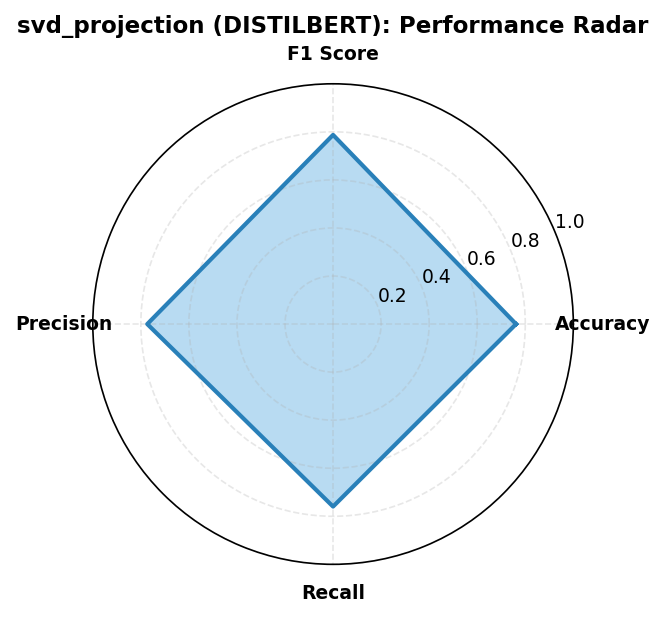
\includegraphics[width=0.85\linewidth]{figures/svd_projection_distilbert_radar_metrics.png}
\caption{Empirical benchmark evaluation and convergence dynamics across models for \texttt{svd_projection_attention}.}
\label{fig:results_svd_projection_attention}
\end{figure}
